\documentclass[10pt,journal,compsoc]{IEEEtran}
\usepackage{blindtext}
\usepackage{graphicx}
\usepackage{multicol}
\usepackage[table,xcdraw]{xcolor}

\ifCLASSOPTIONcompsoc
	\usepackage[caption=false,font=normalsize,labelfont=sf,textfont=sf]{subfig}
\else
	\usepackage[caption=false,font=footnotesize]{subfig}
\fi

\ifCLASSOPTIONcompsoc
	\usepackage[nocompress]{cite}
\else
	\usepackage{cite}
\fi

\ifCLASSINFOpdf
\else
\fi

\newcommand\MYhyperrefoptions{
	bookmarks=true,
	bookmarksnumbered=true,
	pdfpagemode={UseOutlines},
	plainpages=false,
	pdfpagelabels=true,
	colorlinks=true,
	linkcolor={black},
	citecolor={black},
	urlcolor={black},
	pdftitle={Bare Demo of IEEEtran.cls for Computer Society Journals},
	pdfsubject={Typesetting},
	pdfauthor={Michael D. Shell},
	pdfkeywords={Computer Society, IEEEtran, journal, LaTeX, paper, template}
}

\hyphenation{op-tical net-works semi-conduc-tor}


\begin{document}

\title{Design and Simulation of Intellectual Properties Protection using Clipping Filter Algorithm\\with Random Placement
}

\author{
	\begin{multicols}{3}
	Surya Michrandi\\
	School of Electrical Engineering\\
	Telkom University\\
	michrandi@telkomuniversity.ac.id\\

	Fairuz Azmi\\
	School of Electrical Engineering\\
	Telkom University\\
	worldliner@telkomuniversity.ac.id\\

	Hanjara Cahya Adhyatma\\
	School of Electrical Engineering\\
	Telkom University\\
	adhyatma.han@google.com\\
	\end{multicols}
%\IEEEcompsocitemizethanks{
%\IEEEcompsocthanksitem M. Shell was with the Department of Electrical and Computer Engineering, Georgia Institute of Technology, Atlanta, GA, 30332.\protect\\
%E-mail: see http://www.michaelshell.org/contact.html 
%\IEEEcompsocthanksitem J. Doe and J. Doe are with Anonymous University. \IEEEcompsocthanksitem J. Doe and J. Doe are with Anonymous University.} \thanks{Manuscript received April 19, 2005; revised August 26, 2015.}
}

%\markboth{Journal of \LaTeX\ Class Files,~Vol.~14, No.~8, August~2015} {Shell \MakeLowercase{\textit{et al.}}: Bare Advanced Demo of IEEEtran.cls for IEEE Computer Society Journals}

\IEEEtitleabstractindextext{%
\begin{abstract}
System on a Chip (SoC) is an embedded system module that has functionality in a silicon chip board that can also be called Veri Large Scale Integration (VLSI). The owner of the SoC design owns the copyright on the design of the system that has been created. Fabless manufacturing is a way of printing hardware modules that Integrated Circuit (IC) designers are Outsourching from outside the printing factory. Fabless manufacturing from IC design has gap design theft When the design will be printed or when the project requires mutiple module With various functions from various designers. Therefore every module is VLSI Of this chip designer requires proof of ownership of the designer or Production companies. In this study plans to make the verification of ownership design with 2 specific key verification that is Polygate as the main key that will activate the second key, and the second key will be active which process using digital filter algorithm.
\end{abstract}

\begin{IEEEkeywords}
VLSI, Intellectual Property Protection, Digital Signal Processing, Polygate Watermark. 
\end{IEEEkeywords}}

\maketitle
\IEEEdisplaynontitleabstractindextext
\IEEEpeerreviewmaketitle

\ifCLASSOPTIONcompsoc
	\IEEEraisesectionheading{\section{Introduction}\label{sec:introduction}}
\else
	\section{Introduction}
	\label{sec:introduction}
\fi

\IEEEPARstart{P}{roviding} a series of watermarks as a safeguard to a printed VLSI blueprint that indicates ownership of the designer or module manufacturer will protect against cheating others who will steal the design. So the possibility of theft or plagiarism that causes losses to the company or designer because of its design is stolen or plagiarism reduced.\cite{IEEEhowto:kopka}

%\hfill mds
 
%\hfill August 26, 2015

\section{Related Works}
Broadly speaking the technique of Intellectual Property Protection (IPP) watermarking can be classified into 2 classes namely Dynamic Watermarking and Static Watermarking. Dynamic Watermarking is a watermark that can not be detected except by running a watermarked IP to detect the resulting signal, such as digital signal processing (DSP), or finite state mechine (FSM) watermarking. Static Watermarking is a watermark that refers to the properties of a design, and can only be detected in different static ways, such as paths and watermarking placements.[2] One of the other safeguards is to convert the simulated file from a file. The RTL source code that enables is not easy to be reverse-engineered by third parties, so the model can not be changed and reused with other purposes by third parties and irresponsible users. However, this way only protects from the softwere side that protects the IP from being misused by third party users.[3] For IP security used in project sharing and reusable projects can be used with the security of Digital Signal Processing cell that allows integration in the system. In this research will perform a combination of polymorph gate IP protection with digital filter algorithm. Using a combination of these two techniques will provide additional security to IP protection that is likely to over write a smaller watermark. Therefore in this study proposed a combination of existing methods to improve security capabilities in an existing VLSI module. Combine polygate as a combination key to enable the digital filter module to be used as a watermark.

\section{Watermarking}
Providing a series of watermarks as a safeguard to a printed VLSI blueprint that indicates ownership of the designer or module manufacturer will protect against cheating others who will steal the design. So the likelihood of theft or plagiarism is reduced which causes losses to the company or the designer because of his design is stolen or in plagiarism.

\begin{figure}[h]
	\centering
	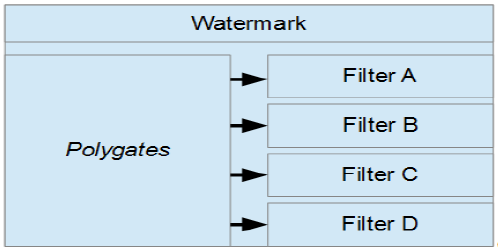
\includegraphics[scale=0.45]{images/box}
	\caption{Simulation results for the network.}
	\label{fig_sim}
\end{figure}

The design will be designed with a combination of Low Pass Filter, High Pass Filter, Band Pass Filter, and Band Reject Filter. This combination will be determined and enabled by polygate as a key to activating a combination of digital filters. After the digital filter is active then the data combination will pass through a combination of filters enabled from the polygate combination.[8], [9] Then the result data combination of these processes will form a special pattern that becomes the watermark data of the designer that characterizes the identity of the designer. Once given the watermark then the module will be tested again its performance. If there is a decrease in performance it should be re-improved the algorithm and then re-tested its performance until obtained the best performance.

\subsection{Polymorph}
\begin{figure}[h]
	\centering
	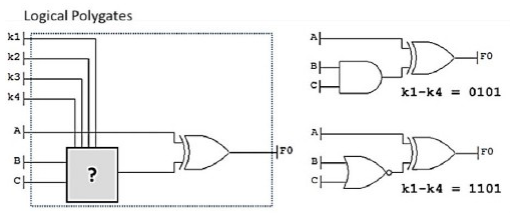
\includegraphics[scale=0.65]{images/polymorphgate}
	\caption{Simulation results for the network.}
	\label{fig_sim}
\end{figure}
Polymorph gate is gate that will change the property of gate such while the key selector key is change. Example is from AND function will active while key is 0101 and it will change to NOR function while key change to 1101.

\subsection{Watermark Flow}
Filter is 3 bit data filter that will clip maximal value or minimal value that has set before. So the data that will go through system is accepted data from clipping filter.
\begin{figure}[h]
	\centering
	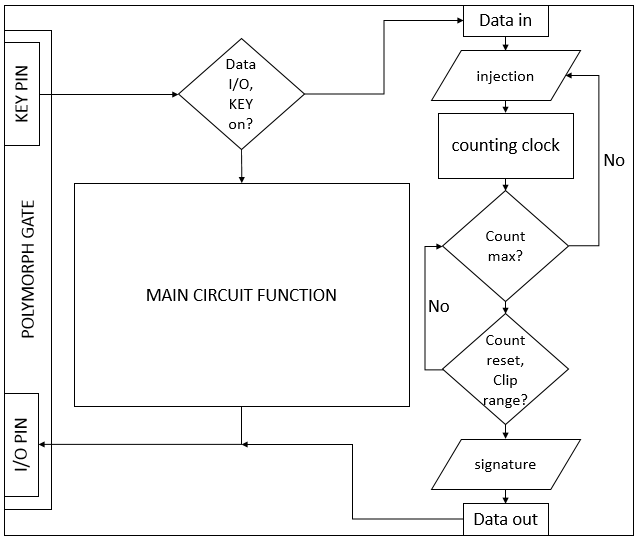
\includegraphics[scale=0.45]{images/flow}
	\caption{Simulation results for the network.}
	\label{fig_sim}
\end{figure}
In this illustration showed how IC is watermarked with given technique. With polymorph gate as bridge between watermark and main circuit function and key pin as gate to access between main function and watermark. To access watermark, developer will activated combined code to given key pin in the printed IC, and after the key activated it will open bridge in the polymorph to watermark circuit. After watermark circuit is opened, developer will inject secret encoded data to circuit and it will decode the given data as signature on the output pin. Data injected as bit stream so it need time to inject and waiting for de-coded output stream.

To extract signature from injected data it will counting how many data will be slice and clip it until given tolerate count. After that data will be checked if the data is inside tolerated range, if yes data will be transferred to polymorph I/O as extracted signature data.

\subsection{Data I/O}
Data in data out is example how filter is going in and let the verification data through system generated and will procced so data will change to specific bit array. By injected long bit stream data to IC with purpose to deceive the attacker. And the output is just specific short bit stream data. The purpose given long input and short output is to avoid watermarks is detected by forced data injection. And here is example with streaming bit data with clipping on the 5/1 injection data. With 20 data stream and 4 data output as zero is ignored. Inputted data will be procced with given algorithm before to extract signature data.
{\renewcommand{\arraystretch}{1.2}
\begin{table}[h]
	\centering
	\caption{Data time verification 20 to 4 clock}
	\label{my-label}
	\begin{tabular}{|
			>{\columncolor[HTML]{EFEFEF}}c |c|c|c|lllll}
		\cline{1-4} \cline{6-9}
		\cellcolor[HTML]{C0C0C0}Time & \cellcolor[HTML]{C0C0C0}in 0 & \cellcolor[HTML]{C0C0C0}in 1 & \cellcolor[HTML]{C0C0C0}in 2 & \multicolumn{1}{c|}{} & \multicolumn{1}{c|}{\cellcolor[HTML]{C0C0C0}Time} & \multicolumn{1}{c|}{\cellcolor[HTML]{C0C0C0}out 0} & \multicolumn{1}{c|}{\cellcolor[HTML]{C0C0C0}out 1} & \multicolumn{1}{c|}{\cellcolor[HTML]{C0C0C0}out 2} \\ \cline{1-4} \cline{6-9} 
		0                            & 1                            & 1                            & 1                            & \multicolumn{1}{c|}{} & \multicolumn{1}{c|}{\cellcolor[HTML]{EFEFEF}0}    & \multicolumn{1}{c|}{0}                             & \multicolumn{1}{c|}{0}                             & \multicolumn{1}{c|}{0}                             \\ \cline{1-4} \cline{6-9} 
		1                            & 1                            & 0                            & 1                            & \multicolumn{1}{c|}{} & \multicolumn{1}{c|}{\cellcolor[HTML]{EFEFEF}1}    & \multicolumn{1}{c|}{0}                             & \multicolumn{1}{c|}{1}                             & \multicolumn{1}{c|}{0}                             \\ \cline{1-4} \cline{6-9} 
		2                            & 1                            & 1                            & 0                            & \multicolumn{1}{c|}{} & \multicolumn{1}{c|}{\cellcolor[HTML]{EFEFEF}2}    & \multicolumn{1}{c|}{0}                             & \multicolumn{1}{c|}{0}                             & \multicolumn{1}{c|}{0}                             \\ \cline{1-4} \cline{6-9} 
		3                            & 0                            & 1                            & 0                            & \multicolumn{1}{c|}{} & \multicolumn{1}{c|}{\cellcolor[HTML]{EFEFEF}3}    & \multicolumn{1}{c|}{0}                             & \multicolumn{1}{c|}{0}                             & \multicolumn{1}{c|}{1}                             \\ \cline{1-4} \cline{6-9} 
		4                            & 0                            & 1                            & 1                            & \multicolumn{1}{l|}{} & \multicolumn{1}{c|}{\cellcolor[HTML]{EFEFEF}4}    & \multicolumn{1}{c|}{0}                             & \multicolumn{1}{c|}{1}                             & \multicolumn{1}{c|}{1}                             \\ \cline{1-4} \cline{6-9} 
		5                            & 1                            & 0                            & 0                            &                       &                                                   &                                                    &                                                    &                                                    \\ \cline{1-4}
		6                            & 0                            & 1                            & 0                            &                       &                                                   &                                                    &                                                    &                                                    \\ \cline{1-4}
		7                            & 0                            & 0                            & 0                            &                       &                                                   &                                                    &                                                    &                                                    \\ \cline{1-4}
		8                            & 1                            & 1                            & 1                            &                       &                                                   &                                                    &                                                    &                                                    \\ \cline{1-4}
		9                            & 1                            & 0                            & 0                            &                       &                                                   &                                                    &                                                    &                                                    \\ \cline{1-4}
		10                           & 0                            & 1                            & 0                            &                       &                                                   &                                                    &                                                    &                                                    \\ \cline{1-4}
		11                           & 0                            & 0                            & 1                            &                       &                                                   &                                                    &                                                    &                                                    \\ \cline{1-4}
		12                           & 0                            & 1                            & 0                            &                       &                                                   &                                                    &                                                    &                                                    \\ \cline{1-4}
		13                           & 1                            & 0                            & 1                            &                       &                                                   &                                                    &                                                    &                                                    \\ \cline{1-4}
		14                           & 0                            & 1                            & 1                            &                       &                                                   &                                                    &                                                    &                                                    \\ \cline{1-4}
		15                           & 1                            & 0                            & 0                            &                       &                                                   &                                                    &                                                    &                                                    \\ \cline{1-4}
		16                           & 0                            & 1                            & 0                            &                       &                                                   &                                                    &                                                    &                                                    \\ \cline{1-4}
		17                           & 1                            & 1                            & 1                            &                       &                                                   &                                                    &                                                    &                                                    \\ \cline{1-4}
		18                           & 0                            & 1                            & 1                            &                       &                                                   &                                                    &                                                    &                                                    \\ \cline{1-4}
		19                           & 0                            & 0                            & 0                            &                       &                                                   &                                                    &                                                    &                                                    \\ \cline{1-4}
	\end{tabular}
\end{table}
}


\subsection{Layouting}
Gate for layout use CMOS technology. The protection use simple basic CMOS gate for mixed implemented for hard removal from reverse engineering, there are:
\begin{figure}[h]
	\centering
	\subfloat[Case I]{
		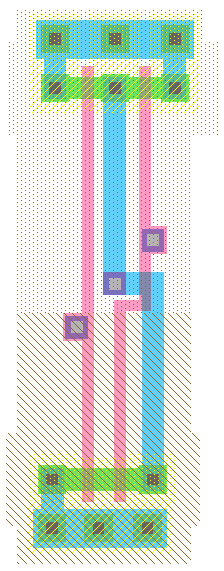
\includegraphics[width=0.9in]{images/gateNAND} \label{fig_first_case}}
	\hfil
	\subfloat[Case II]{
		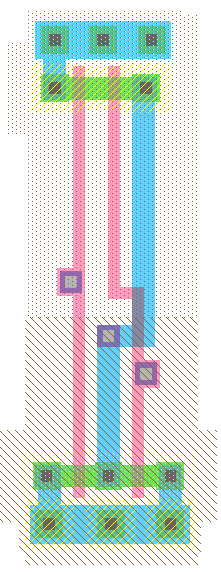
\includegraphics[width=0.9in]{images/gateNOR} \label{fig_second_case}}
	\hfil
	\subfloat[Case III]{
		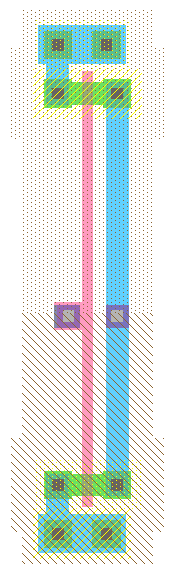
\includegraphics[width=0.9in]{images/gateNOT} \label{fig_second_case}}
	\caption{Simulation results for the network.}
	\label{fig_sim}
\end{figure}
\subsection{Layout Verification}
For simple see through layout with just verification without mixed gate placement, here is total gate if the gate collected as one cell:
\begin{figure}[h]
	\centering
	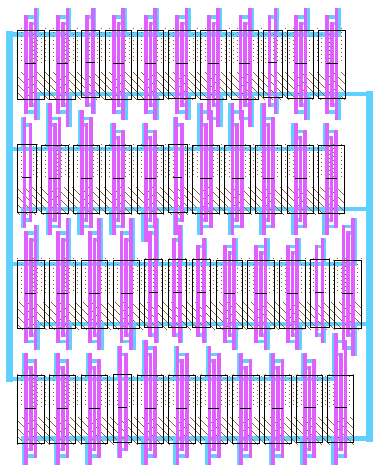
\includegraphics[scale=0.8]{images/gate1}
	\caption{Simulation results for the network.}
	\label{fig_sim}
\end{figure}
\subsection{Mixed Random Gate Placement}
In general technique when engineer will manufacturing IC is make hierarchy of cells so it will easy to routing and tracing circuit problem. But if the watermark circuit is manufactured with that technique it will easy to expose watermark circuit inside the IC. So it will lead to hard removal and reverse engineered the IC. To prevent that happening the watermark cell will generate without hierarchy and placed with random routing algorithm. So it will not be so obvious that watermark’s circuit is implemented within the main IC core circuit.
\begin{figure}[h]
	\centering
	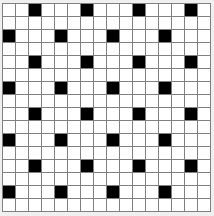
\includegraphics[scale=1.0]{gatePlace}
	\caption{Simulation results for the network.}
	\label{fig_sim}
\end{figure}
Mixed Random Gate Placement is randomize Verification’s components with main IP cell component. So it will placed wherever inside IP cell. Here is figure that tell how verification’s components gate placed inside main IP cell:

%\begin{figure}[!t]
%	\centering
%	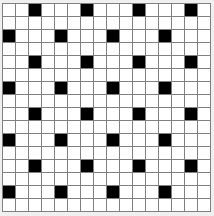
\includegraphics[width=2.5in]{gatePlace}
%	\caption{Simulation results for the network.}
%	\label{fig_sim}
%\end{figure}

%\begin{figure*}[!t]
%	\centering
%	\subfloat[Case I]{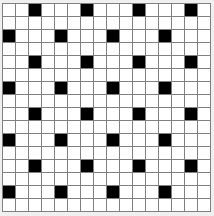
\includegraphics[width=2.5in]{gatePlace} \label{fig_first_case}}
%	\hfil
%	\subfloat[Case II]{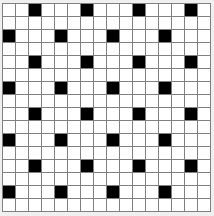
\includegraphics[width=2.5in]{gatePlace} \label{fig_second_case}}
%	\caption{Simulation results for the network.}
%	\label{fig_sim}
%\end{figure*}

The dark dot representation of NAND, NOR and INVERTER from verification components. So for hard removal watermark it will change entire design and it will harder to detect watermark from random placement.

\section{Analysis}
In this section, analysis is focution on how watermark actualy didn't create error to original design
so watermark will be usefull to protect original design from thiefing.

\subsection{Watermark softwere simulation}
This is simulation from data given before. Data from device to read and inject data is translated as alphabetic character from 3 bits data stream. It is show long data stream with short data output as signature.
{\renewcommand{\arraystretch}{1.2}
\begin{table}[h]
	\centering
	\caption{Input Array}
	\label{inputarray}
	\begin{tabular}{|c|c|}
		\hline
		H                            & 111                                      \\ \hline
		F                            & 101                                      \\ \hline
		G                            & 110                                      \\ \hline
		C                            & 010                                      \\ \hline
		D                            & 011                                      \\ \hline
		E                            & 100                                      \\ \hline
		C                            & 010                                      \\ \hline
		A                            & 000                                      \\ \hline
		H                            & 111                                      \\ \hline
		E                            & 100                                      \\ \hline
		C                            & 010                                      \\ \hline
		B                            & 001                                      \\ \hline
		C                            & 010                                      \\ \hline
		F                            & 101                                      \\ \hline
		D                            & 011                                      \\ \hline
		E                            & 100                                      \\ \hline
		C                            & 010                                      \\ \hline
		H                            & 111                                      \\ \hline
		D                            & 011                                      \\ \hline
		\multicolumn{1}{|l|}{INPUT}  & \multicolumn{1}{l|}{HFGCDECAHECBCFDECHD} \\ \hline
		\multicolumn{1}{|l|}{OUTPUT} & \multicolumn{1}{l|}{CABE}                \\ \hline
	\end{tabular}
\end{table}
}

\subsection{Power Consumption Orogonal Design}
Power consumption is the most important thing in the electronic design, adding more component
mean more power is needded to drive the device. Here data from experiment with original design
in power consumption needed to drive the device:
{\renewcommand{\arraystretch}{1.2}
\begin{table}[h]
	\centering
	\caption{Original Power}
	\label{my-label}
	\begin{tabular}{|c|c|c|c|}
		\hline
		\rowcolor[HTML]{C0C0C0} 
		\begin{tabular}[c]{@{}c@{}}Supply\\ Source\end{tabular} & \begin{tabular}[c]{@{}c@{}}Supply\\ Voltage\end{tabular} & \begin{tabular}[c]{@{}c@{}}Total\\ Current\\ (mA)\end{tabular} & \begin{tabular}[c]{@{}c@{}}Quiescent\\ Current\\ (mA)\end{tabular} \\ \hline
		\cellcolor[HTML]{EFEFEF}Vccint                          & 1.2                                                      & 2.01                                                           & 2.01                                                               \\ \hline
		\cellcolor[HTML]{EFEFEF}Vccaux                          & 2.5                                                      & 3.00                                                           & 3.00                                                               \\ \hline
		\cellcolor[HTML]{EFEFEF}Vcco25                          & 2.5                                                      & 0.20                                                           & 0.20                                                               \\ \hline
	\end{tabular}
\end{table}
}

\subsection{Power Consumption Watermark}
Power consumption is the most important thing in the electronic design, adding more component
mean more power is needded to drive the device. Here data from experiment with original design
in power consumption needed to drive the device:
{\renewcommand{\arraystretch}{1.2}
	\begin{table}[h]
		\centering
		\caption{Watermark Power}
		\label{watermark}
		\begin{tabular}{|c|c|c|c|}
			\hline
			\rowcolor[HTML]{C0C0C0} 
			\begin{tabular}[c]{@{}c@{}}Supply\\ Source\end{tabular} & \begin{tabular}[c]{@{}c@{}}Supply\\ Voltage\end{tabular} & \begin{tabular}[c]{@{}c@{}}Total\\ Current\\ (mA)\end{tabular} & \begin{tabular}[c]{@{}c@{}}Quiescent\\ Current\\ (mA)\end{tabular} \\ \hline
			\cellcolor[HTML]{EFEFEF}Vccint                          & 1.2                                                      & 2.89                                                           & 2.01                                                               \\ \hline
			\cellcolor[HTML]{EFEFEF}Vccaux                          & 2.5                                                      & 3.00                                                           & 3.00                                                               \\ \hline
			\cellcolor[HTML]{EFEFEF}Vcco25                          & 2.5                                                      & 0.20                                                           & 0.20                                                               \\ \hline
		\end{tabular}
	\end{table}
}
%////////////////////////////////////////////////////////////////////////////////////
% COMPARISON
%////////////////////////////////////////////////////////////////////////////////////
\subsection{Comparison}
On the Table 2 are comparison about all parameter that tested on
{\renewcommand{\arraystretch}{1.2}
\begin{table}[h]
	\centering
	\caption{Comparison}
	\label{comparison}
	\begin{tabular}{|c|c|c|c|c|}
		\hline
		\rowcolor[HTML]{C0C0C0} 
		No.                        & Parameter  & Before & After  & Delta \\ \hline
		\cellcolor[HTML]{EFEFEF}1. & Gates      & 5234   & 5324   & 1.72  \\ \hline
		\cellcolor[HTML]{EFEFEF}2. & Layout     & Lamda  & lamda  &       \\ \hline
		\cellcolor[HTML]{EFEFEF}3. & Power      & A      & A      &       \\ \hline
		\cellcolor[HTML]{EFEFEF}4. & Functional & Normal & Normal & zero  \\ \hline
	\end{tabular}
\end{table}
}
%////////////////////////////////////////////////////////////////////////////////////
% KESIMPULAN
%////////////////////////////////////////////////////////////////////////////////////
\section{Conclusion}
From the experiment testing for performance analysis with given parameter. The percentage change is still within reasonable limits. So that in its application still can be applied.
%\begin{figure*}[!h]
%	\centering
%	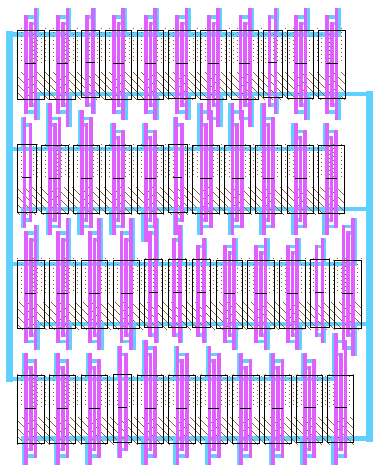
\includegraphics[scale=1.7]{images/gate1}
%	\caption{Simulation results for the network.}
%	\label{fig_sim}
%\end{figure*}

\appendices
\section{Proof of the First Zonklar Equation}
Appendix one text goes here.

\section{}
Appendix two text goes here.

\ifCLASSOPTIONcompsoc
  \section*{Acknowledgments}
\else
  \section*{Acknowledgment}
\fi

The authors would like to thank...

\ifCLASSOPTIONcaptionsoff
  \newpage
\fi

\begin{thebibliography}{1}

\bibitem{IEEEhowto:kopka}
H.~Kopka and P.~W. Daly, \emph{A Guide to {\LaTeX}}, 3rd~ed.\hskip 1em plus
0.5em minus 0.4em\relax Harlow, England: Addison-Wesley, 1999.

\bibitem{chapman}
R. Chapman and T. S. Durrani, “IP Protection of DSP Algorithms for System on Chip Implementation,” vol. 48, no. 3, pp. 854–861, 2000.

\bibitem{water}
“Watermarking Techniques for Electronic Circuit Design,” no. 1, pp. 1–17.

\bibitem{lui}
Q. Liu, W. Ji, Q. Chen, and T. Mak, “IP Protection of Mesh NoCs Using Square Spiral Routing,” vol. 24, no. 4, pp. 1560–1573, 2016.

\bibitem{cui}
A. Cui, C. Chang, S. Member, S. Tahar, and S. Member, “A Robust FSM Watermarking Scheme for IP Protection of Sequential Circuit Design,” vol. 30, no. 5, pp. 678–690, 2011.

\bibitem{nie}
T. Nie, “Performance Evaluation for IP Protection Watermarking Techniques.”

\bibitem{zhang1}
J. Zhang, Y. Lin, Y. Lyu, G. Qu, and S. Member, “A PUF-FSM Binding Scheme for FPGA IP Protection and Pay-Per-Device Licensing,” vol. 10, no. 6, pp. 1137–1150, 2015.

\bibitem{zhang2}
J. Zhang, Y. Lin, Q. Wu, and W. Che, “Watermarking FPGA Bitfile for Intellectual Property Protection,” pp. 764–771.

\bibitem{kahng}
A. B. Kahng et al., “Watermarking Techniques for Intellectual Property Protection.”

\bibitem{mosh}
V. G. Moshnyaga and H. Nita, “STG-based Detection of Power Virus Inputs in FSM.”



\end{thebibliography}

\begin{IEEEbiography}[{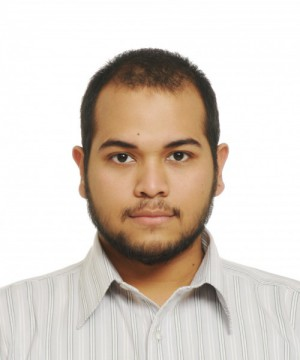
\includegraphics[width=1in,height=1.25in,clip,keepaspectratio]{./images/paksurya}}]{Surya Michrandi}
\blindtext[1]
\end{IEEEbiography}

\begin{IEEEbiography}[{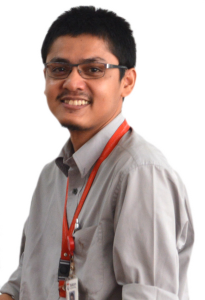
\includegraphics[width=1in,height=1.25in,clip,keepaspectratio]{./images/pakazmi}}]{Fairuz Azmi}
\blindtext[1]
\end{IEEEbiography}

\begin{IEEEbiography}[{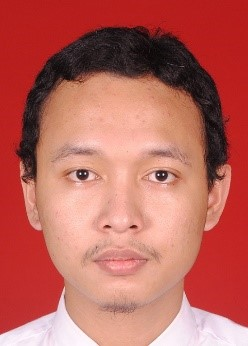
\includegraphics[width=1in,height=1.25in,clip,keepaspectratio]{./images/hanjara}}]{Hanjara Cahya Adhyatma}
\blindtext[1]
\end{IEEEbiography}

\end{document}


